\documentclass[ 12pt, a4paper]{article}
% Use the option doublespacing or reviewcopy to obtain double line spacing
% \documentclass[doublespacing]{elsart}

\usepackage[utf8]{inputenc}

\usepackage[style= bwl-FU, backend = biber, maxcitenames=2,uniquelist=minyear]{biblatex}
\addbibresource{MultipleScattering.bib}

\usepackage{color,graphicx,tikz}
\usetikzlibrary{positioning,arrows}
% The amssymb package provides various useful mathematical symbols
\usepackage{mathtools,amssymb,amsmath,mathdots}
\usepackage[mathscr]{eucal} %just for the font \mathscr
\usepackage{enumerate}
\usepackage{setspace}
\usepackage{hyperref}

% macros used across many documents for multiple scattering notation
%% Packages for commenting and striking through text %%%%
\usepackage[colorinlistoftodos,bordercolor=orange,backgroundcolor=orange!20,linecolor=orange,textsize=scriptsize]{todonotes}
\usepackage{soul}
\newcommand{\will}[1]{\todo[inline]{\textbf{Will: }#1}}
\newcommand{\art}[1]{\todo[inline]{\textbf{Art: }#1}}
\newcommand{\david}[1]{\todo[inline]{\textbf{David: }#1}}
\newcommand{\mike}[1]{\todo[inline]{\textbf{Mike: }#1}}
\newcommand{\wrong}[1]{\textcolor{red}{\st{#1}}}
%%%--------------------------------------------------%%%

\newcommand \eff {*}
\newcommand \scatZ {Z}
\newcommand \scatZs {\zeta}
\newcommand \Q {\vec Q}
\newcommand \T {\vec T}
\newcommand \B {\mathcal B}
\newcommand \regS {\mathcal S}
\newcommand \M {\vec {\mathcal M}}
\newcommand \s {\mathbf s}
\newcommand \Ab {\mathcal A}
\newcommand \A [1] {\Ab_#1}
\newcommand \p {p}
\newcommand \prob {P}
\newcommand {\type} [1]{{\{#1\}}}
\newcommand \reg {\mathcal R_N}
\newcommand \reginf {\mathcal R_\infty}
\newcommand {\nfrac}[1] {\mathfrak n_{#1}}
\newcommand {\Lamo}{\vec \Lambda}
\newcommand {\Lam}[1]{\Lamo_{#1}}
\newcommand \ef{\mathrm{E}}
\newcommand \reflect{\mathrm{ref}}
\newcommand \inc{\mathrm{in}}
\newcommand \In{\mathrm{I}}
\newcommand \cs { S}
\newcommand \cl { L}
\newcommand \Out{\mathrm{o}}

% \newcommand \nfrac {\mathfrak n_0}
\newcommand{\ensem}[1]{\langle #1 \rangle}

\def\bga#1\ega{\begin{gather}#1\end{gather}} % suggested in technote.tex
\def\bgas#1\egas{\begin{gather*}#1\end{gather*}}

\def\bal#1\eal{\begin{align}#1\end{align}} % suggested in technote.tex
\def\bals#1\eals{\begin{align*}#1\end{align*}}

\renewcommand{\vec}[1]{\boldsymbol{#1}}
\renewcommand{\thefootnote}{\fnsymbol{footnote}}

\newcommand{\initial}[1]{{#1}_\circ}
\newcommand{\ii}{\textrm{i}}
\newcommand{\ee}{\textrm{e}}
\newcommand{\deriv}[2]{\frac{\partial{#1}}{\partial{#2}}}
\newcommand{\derivtwo}[2]{\frac{\partial^{2}{#1}}{\partial{#2}^2}}
\newcommand{\derivtwomix}[3]{\frac{\partial^{2}{#1}}{\partial{#2}\partial{#3}}}

\newcommand{\bb}{\mathcal B}
\newcommand{\R}{\mathbb{R}}
\newcommand{\filler}{\hspace*{\fill}}

\newcommand{\lit}{\hspace{0.2cm}}

\newtheorem{theorem}{Theorem}
\def \proof{\noindent {\bf \emph{Proof:}} }


% \DeclareMathOperator{\sign}{sgn}
% \DeclareMathOperator{\divergence}{div}
% \DeclareMathOperator{\tr}{tr}
% \DeclareMathOperator{\Ord}{\mathcal{O}}
% \DeclareMathOperator{\GRAD}{grad}
% \DeclareMathOperator{\DIV}{DIV}
% \DeclarePairedDelimiter{\ceil}{\lceil}{\rceil}


%%% Local Variables:
%%% mode: latex
%%% TeX-master: t
%%% End:


\renewcommand {\Lam}[1]{\mathbf x_{#1}}

% \graphicspath{{../images/}}

\doublespacing
% \setlength{\topmargin}{0cm} \addtolength{\textheight}{2cm}
\evensidemargin=0cm \oddsidemargin=0cm \setlength{\textwidth}{16cm}

\begin{document}

\title{Average reflection from a random particulate material}
\author{
Artur L. Gower$^{a}$ \\[12pt]
% , William Parnell$^{a}$ and David Abrahams$^{b}$ \\[12pt]
\footnotesize{$^{a}$ School of Mathematics, University of Manchester, Oxford Road, Manchester, M13 9PL,UK}\\
% \footnotesize{$^{b}$ School of Oo La la Cambridge}
}
\date{\today}
\maketitle

\begin{abstract}
Does a halfspace filled with randomly placed cylinders behave, on average, like a homogeneous halfspace? To answer this, we compare the reflection from a homogeneous halfspace with the average reflection from a halfspace filled with cylinders. In the end we reach an absurd result for cylinders with Dirichlet boundary condition. An explanation for this absurd result would be great.
\end{abstract}

\noindent
{\textit{Keywords:} blue sky thinking}

\section{Reflection from a halfspace}

We consider an incident plane wave
\[
u_\inc(x,y) = \ee^{\ii (\alpha x + \beta y)}, \quad \text{with} \;\; (\alpha,\beta) = k ( \cos \theta_\inc,  \sin \theta_\inc),
\]
and assume time-harmonic dependence of the form $\ee^{-\ii \omega t}$. The incident wave $u_\inc(x,y)$ is heading towards the interface $ x=0$, which divides two homogeneous materials. The material on the left (right) has wavenumber and density $k$ and $\rho$ ($k_\eff$ and $\rho_\eff$). The reflected and transmitted wave will be of the form
\[
u_R = R \ee^{\ii ( - x \alpha + y \beta)} \quad \text{and} \quad
u_T = T \ee^{\ii (x \alpha_\eff + y \beta_\eff)},
\]
where $k_\eff(\cos \theta_\eff,\sin \theta_\eff) = ( \alpha_\eff, \beta_\eff)$.

The boundary conditions for the acoustic pressure are
\[
u_\inc + u_R = u_T \quad \text{and} \quad  \frac{1}{\rho}\frac{\partial u_\inc}{\partial x} + \frac{1}{\rho}\frac{\partial u_R}{\partial x} = \frac{1}{\rho_\eff}\frac{\partial u_T}{\partial x}, \quad \text{for} \quad x=0,
\]
from which we get Snell's law
\begin{equation}
k \sin \theta_\inc = k_\eff \sin \theta_\eff,
\label{eqn:Snells}
\end{equation}
and
\begin{equation}
  R = \frac{q_\eff \cos \theta_\inc - \cos \theta_\eff}{q_\eff \cos \theta_\inc + \cos \theta_\eff}, \quad 
  T = \frac{2q_\eff \cos \theta_\inc}{q_\eff \cos \theta_\inc + \cos \theta_\eff},
  \quad \text{with} \quad q_\eff = \frac{k \rho_\eff}{k_\eff \rho}.
  \label{eqn:Reflection}
\end{equation}
Note that $1 + R = T$.

From this we can establish bounds such as $|R|\leq 1$, can you prove this? What happens when $k_\eff$ is a complex number? Later, we will see that the reflection coefficient from a random mix of cylinders (with Dirichlet boundary condition), is unbounded! And the problem is in the limit for small $k$. This is likely wrong, and we are not sure why.


\section{Reflection from multiple random cylinders}

\subsection{Multipole method for cylinders}

Here we give the exact theory for scalar multiple wave scattering from a finite number $N$ of circular cylinders. The pressure $u$ outside all the cylinders satisfies the scalar Helmholtz equation
\be
\nabla^2 u + k^2 u = 0,
% c^2 \nabla^2 u + \omega^2 u = 0,
\en
and inside the $j$th cylinder the pressure $u_j$ satisfies
\be
  \nabla^2 u_j + k^2_o u_j = 0, \quad \text{for} \; j=1,2,\ldots, N,
  % c_j^2 \nabla^2 u_j + \omega^2 u_j = 0, \quad \text{for} \; j=1,2,\ldots, N,
	% \\
  % c_{N_\cs + 1}^2 \nabla^2 u^{N_\cs +j} + \omega^2 u^{N_\cs +j} = 0 \quad \text{for} \; j= 1, 2,\ldots, N_\cl
\en

where $\nabla^2$ is the two-dimensional Laplacian and
\be \label{eqns:wavenumbers}
	k = \omega/c \quad \text{and} \quad k_o = \omega/c_o.
\en
% where $\omega$ is the angular frequency and we have implicitly specified a time dependence of $\ee^{-\ii \omega t}$.

\begin{figure}[t]
  \centering
  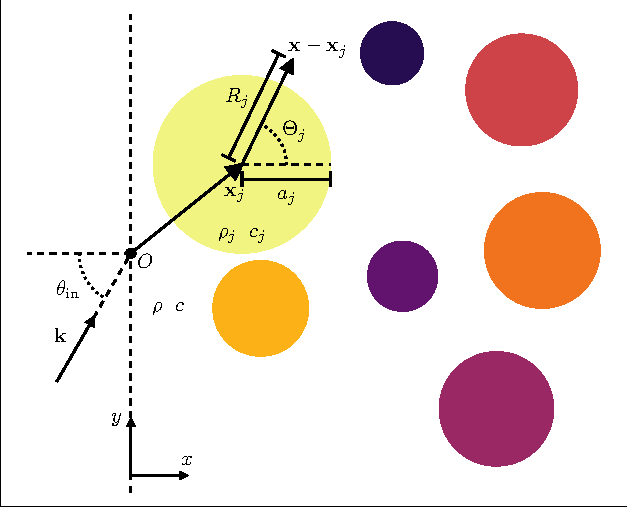
\includegraphics[width=0.72\linewidth]{multispecies.pdf}
  \caption{ represents a multi-species material comprising different species of cylinders to the right of the origin $O = (0,0)$. The vector $\mathbf x_j$ points to the centre of the $j$-th cylinder, with a local polar coordinate system $(R_j, \Theta_j)$. Each cylinder has a radius $a_j$, density $\rho_j$, and wave speed $c_j$, while the background has density $\rho$ and wave speed $c$. The vector $\mathbf k$ is the direction of the incident plane wave.  }
  \label{fig:multispecies}
\end{figure}

We use for each cylinder the polar coordinates
\be
R_{j} =\| \mathbf x- \mathbf x_{j} \|, \quad \Theta_{j} = \arctan\left ( \frac{y-y_{j}}{x- x_{j}} \right),
\label{eqns:polar_coords}
\en
where $\mathbf x_j$ is the centre of the $j$-th cylinder and $\mathbf x = (x,y)$ is an arbitrary point with origin $O$. See Figure~\ref{fig:multispecies} for a schematic of the material properties and coordinate systems.
Then we can define $u_j$ as the scattered pressure field from the $j$-th cylinder,
\bga \label{eqn:outwaves}
	u_j(R_j,\Theta_j) = \sum_{m=-\infty}^\infty A_j^m Z^m H_m(k R_j) \ee^{\ii m \Theta_j}, \quad \text{for} \;\; R_j > a_j,
\ega
where $H_m$ are Hankel functions of the first kind, $A_j^m$ are arbitrary coefficients and $Z^m$ characterises the type of scatterer:
\be
Z^m = \frac{q J_m' (k a) J_m ({k_o} a) - J_m (k a) J_m' ({k_o} a) }{q H_m '(k a) J_m({k_o} a) - H_m(k a) J_m '({k_o} a)} = Z^{-m},
\label{eqn:Zm}
\en
with ${q} = (\rho_o k)/(\rho k_o)$. In the limits ${q} \to 0$ or ${q} \to \infty$, the coefficients for Dirichlet or Neumann boundary conditions are recovered, respectively.


The pressure outside all cylinders is the sum of the incident wave $u_\inc$ and all scattered waves,
\be \label{eq:totwave}
u(x,y) =
% u_\inc(x,y)  + u_\mathrm{scatt}(x,y)  =
  u_\inc(x,y) +\sum_{j=1}^N u_j(R_j,\Theta_j).
\en
and the total field inside the $j$-th cylinder is
\be \label{eqn:inwaves}
u_{j}^\In(R_j,\Theta_j) = \sum_{m=-\infty}^\infty B_j^m J_m(k_j R_j) \ee^{\ii m \Theta_j}, \quad \text{for} \;\; R_j < a_j.
\en

The unknown coefficients are determined through the boundary conditions of continuity of pressure and normal   velocity on the cylinder boundaries:
\be \label{eqn:BC}
	u = u^\In_{j} \quad \text{and} \quad \frac{1}{\rho} \frac{\partial u}{\partial R_j} = \frac{1}{\rho_o} \frac{\partial u^\In_{j}}{\partial R_j}, \quad \text{on} \;\; R_j = a\;\; \text{for} \; \; j=1, \ldots, N.
\en

When the cylinders are far apart, the solution for the $A_j^m$ are similar to the solution for one lone cylinder scattering the incident wave $u_\inc$, which is
\begin{equation}
A^m_j = -\ii^m \ee^{-\ii m \theta_\inc} \ee^{\ii \mathbf x_j \cdot \mathbf k}.
\label{eqn:SingleScatterer}
\end{equation}
Using the above and assuming the cylinders are far apart, the scattered field far away from the cylinder~\eqref{eqn:outwaves} becomes
\begin{equation}
    \lim_{R_j \to \infty} u_j(R_j,\Theta_j)
% = -\lim_{R_j \to \infty} \sum_{m=-\infty}^\infty \ii^m \ee^{-\ii m \theta_\inc} \ee^{\ii \mathbf x_j \cdot \mathbf k} Z^m H_m(k R_j) \ee^{\ii m \Theta_j} \\
    \sim \sqrt{\frac{2}{\pi k R_j}} f_\circ(\Theta_j-\theta_\inc)\ee^{\ii k R_j -\ii \pi/4},
\end{equation}
where
\begin{equation}
 f_\circ(\theta) = - \sum_{m=-\infty}^\infty \ee^{\ii m \theta} \scatZ^m.
 \label{eqn:FarField}
\end{equation}

\subsection{Ensemble average}

For an introduction to ensemble-averaging of multiple scattering see~\cite{foldy_multiple_1945}.

Consider a configuration of $N$ circular cylinders centred at $\mathbf x_1,\mathbf x_2, \ldots, \mathbf x_N$. Each $\mathbf x_j$ is in the region $\reg$, where $\nfrac {} = N/|\reg|$ is the total number density and $|\reg|$ is the area of $\reg$.
The probability of the cylinders being in a specific configuration is given by the probability density function $\p(\mathbf x_1,\mathbf x_2,\ldots, \mathbf x_N)$, so that
\be
\int \p(\mathbf x_1) d \mathbf x_1 = \int \int \p(\mathbf x_1, \mathbf x_2) d \mathbf x_1 d \mathbf x_2 = \ldots = 1.
\en
And as the cylinders are indistinguishable: $\p(\mathbf x_1, \mathbf x_2) = \p(\mathbf x_2, \mathbf x_1)$.

Furthermore, we have
\bal
  &\p(\mathbf x_1, \ldots, \mathbf x_N) = \p(\mathbf x_j) \p(\mathbf x_{1}, \ldots, \mathbf x_N|\mathbf x_j),
  \label{eqns:conditional_probj}
  \\
  &\p(\mathbf x_1, \ldots, \mathbf x_N|\mathbf x_j) = \p(\mathbf x_\ell |\mathbf x_j) \p( \mathbf x_1, \ldots, \mathbf x_N|\mathbf x_\ell,\mathbf x_j),
  \label{eqns:conditional_probsj}
\eal
where $\p(\mathbf x_{1}, \ldots, \mathbf x_N|\mathbf x_j)$ is the conditional probability of having cylinders centred at $\mathbf x_{1}, \ldots, \mathbf x_N$ (not including $\mathbf x_j$), given that the $j$-th cylinder is fixed at $\mathbf x_j$. Likewise, $\p( \mathbf x_1, \ldots, \mathbf x_N| \mathbf x_{\ell},\mathbf x_{j})$ is the conditional probability of having cylinders centred at $\mathbf x_{1}, \ldots, \mathbf x_N$ (not including $\mathbf x_\ell$ and $\mathbf x_j$) given that there are already two cylinders centred at $\mathbf x_\ell$ and $\mathbf x_j$.

Given some function $F(\mathbf x_{1}, \ldots, \mathbf x_{N})$, we denote its average, or {\it expected value}, by
\be
\ensem F  = \int\ldots \int F(\mathbf x_{1}, \ldots, \mathbf x_{N}) \p(\mathbf x_{1}, \ldots, \mathbf x_{N}) d\mathbf x_{1} \ldots d\mathbf x_{N} .
\en
If we fix the location and properties of the $j$-th cylinder, $\mathbf x_{j}$  and average over all the properties of the other cylinders, we obtain a {\it conditional average} of $F$ given by
\be
\ensem{F}_{\mathbf x_{j}} = {\int\ldots} \int F(\mathbf x_{1}, \ldots, \mathbf x_{N}) \p( \mathbf x_{1}, \ldots, \mathbf x_{N}|\mathbf x_{j}) d  \mathbf x_{1} \ldots \mathbf x_N,
\en
where we do not integrate over $\mathbf x_j$. The average and conditional averages are related by
\bga
\ensem{F}  =   \int  \ensem{F}_{\mathbf x_j} \p(\mathbf x_j) \, d \mathbf x_j \quad \text{and} \quad \ensem{F}_{\mathbf x_j} =  \int  \ensem{F}_{ \mathbf x_j \mathbf x_\ell} \p(\mathbf x_\ell)\, d \mathbf x_\ell,
\label{eqns:conditional_averages}
\ega
where $\ensem{ F}_{\mathbf x_\ell\mathbf x_j}$ is the conditional average when fixing both $\mathbf x_j$ and $\mathbf x_\ell$, and $\ensem{ F}_{\mathbf x_\ell\mathbf x_j} = \ensem{ F}_{\mathbf x_j \mathbf x_\ell}$.

We can now calculate the average total pressure (incident plus scattered), measured at some position $\mathbf x$ outside of $\reg$, by averaging~\eqref{eq:totwave} to obtain
\be
\ensem{u(x,y)} = u_\inc(x,y) + \sum_{j=1}^N \int \ldots \int u_j(R_j,\Theta_j) \p(\mathbf x_1, \ldots, \mathbf x_N) d \mathbf x_1 \ldots d \mathbf x_N,
\en
where $\ensem{u_\inc(x,y)} = u_\inc(x,y)$, because the incident field is independent of the scattering configuration.
% , and $r_1$ and $\theta_1$ depend on $\mathbf x_1$ and $\mathbf x$ through the definitions~\eqref{eqns:polar_coords}.
We can then rewrite the average outgoing wave $u_j$ by fixing the properties of the $j$-th cylinder $\mathbf x_j$ and using equation~\eqref{eqns:conditional_probj} to reach
\bal
  \ensem{u(x,y)} -u_\inc(x,y) =&  \sum_{j=1}^N \int \ensem{u_j(R_j,\Theta_j)}_{\mathbf x_j} \p(\mathbf x_j) d \mathbf x_j
  %  \notag \\
  =  N \int \ensem{u_1(R_1,\Theta_1)}_{\mathbf x_1} \p(\mathbf x_1) d \mathbf x_1.
\label{eqn:AverageWave}
\eal
% as the average outgoing wave from any one of the cylinders.
% Said another way, $\mathbf x_j$ was a dummy variable in equation~\eqref{eqn:AverageWave} that was changed to $\mathbf x_1$.
Likewise, for the conditionally averaged scattered field~\eqref{eqn:outwaves} measured at $\mathbf x$ we obtain
\bga
	% \ensem{u_j(r_j,\theta_j)}_{\mathbf x_j} = \sum_{m=-\infty}^\infty \ensem{A_j^m}_{\mathbf x_j} \scatZ^m_j H_m^{(1)}(k r_j) \ee^{\ii m \theta_j},
	\ensem{u_1(R_1,\Theta_1)}_{\mathbf x_1} = \sum_{m=-\infty}^\infty \ensem{A_1^m}_{\mathbf x_1} \scatZ^m H_m^{(1)}(k R_1) \ee^{\ii m \Theta_1}.
\label{eqn:AverageWaveCond}
\ega

We will use the simplest approximations possible, which are a random uniform distribution
\be
\p(\Lam 1) = \frac{1}{|\reg|},
\label{eqn:pLam1}
\en
which combined with~\eqref{eqn:AverageWave} and \eqref{eqn:AverageWaveCond}, and taking the limit $N \to \infty$ with ${\reg}$ turning into a halfspace $x_1>0$, leads to
\begin{equation}
  \ensem{u(x,y)} = u_\inc(x,y)+   \nfrac {} \sum_{m=-\infty}^\infty \scatZ^m \int_{x_1>0}   \ensem{A_1^m}_{\mathbf x_1}  H_m^{(1)}(k R_1) \ee^{\ii m \Theta_1}  d \mathbf x_1.
  \label{eqn:AverageReflection}
\end{equation}
When $x <0$, the above turns into the incident wave plus the average reflected field from the halfspace $x>0$.

\subsection{Effective medium approach}

The simplest approach is to assume that, on average, the wave exciting a scatterer is a plane wave.
That is, for $x_1 > 0$, we assume
\begin{align}
  \ensem{A_1^m}_{\mathbf x_1} =  \ii^m \ee^{-\ii m \theta_\eff} \A m_\eff \ee^{\ii \mathbf x \cdot \mathbf k_\eff}, \quad \text{for} \quad x>{0},
  \label{eqn:AnsatzA}
\end{align}
where the constant factor $\ii^m \ee^{-\ii m \theta_\eff}$ is just for later convenience, $\A m_\eff$ is an unknown constant (for now), and we define
\begin{equation}
  \mathbf k_\eff =(\alpha_\eff, \beta) := k_\eff(\cos\theta_\eff, \sin\theta_\eff),
\end{equation}
and from Snell's law
\begin{equation}
  k_\eff \sin \theta_\eff = k \sin \theta_\inc,
  \label{eqn:Snells}
\end{equation}
  noting that both $\theta_\eff$ and $k_\eff$ are complex numbers.

\begin{align}
    & \A m_\eff(\s_1)  +  2 \pi \nfrac {} \sum_{n=-\infty}^\infty\int_\regS  \A n_\eff(\s_2)
  \left [ \frac{\mathcal N_{n-m}(ka_{12},k_\eff a_{12})}{k^2 - k_\eff^2} \right]
    d\s_2^n
   = 0,
 \label{eqn:AmT}
\\
  &
   \sum_{n=-\infty}^\infty \ee^{\ii n (\theta_\inc - \theta_\eff)} \int_\regS
   \A n_\eff(\s_2) d\s_2^n = (\alpha_\eff-\alpha) \frac{\alpha \ii}{2 \nfrac {} },
 \label{eqn:AmInc}
 \end{align}
 where
\begin{equation}
  d \s_2^n = Z^n(\s_2) p(\s_2) d\s_2,
\end{equation}
 % $a_2$ is the radius of the $s_2$ specie,
 we used whole-correction and ignored the boundary layer (which disappears in the low-frequency limit anyway). The above equations are sufficient to completely determine $k_\eff$ and $\A n_\eff$.

First using $k_\eff = c k /c_\eff $:
\[
 \mathcal N_{n}(ka_{12},k_\eff a_{12}) \sim \frac{2 \ii c^{|n|}}{\pi c_\eff^{|n|}} + \mathcal O(k^2),
\]
because this does not depend on the species, we can move it outside the integral in~\eqref{eqn:AmT}, multiple $Z^m(\s_1) p(\s_1)$ on both sides of the equation  and then integrate in $\s_1$ to reach,
\begin{align}
    & \ensem{\A m_\eff}^m  +  \frac{4 \ii \nfrac {}}{k^2} \frac{c_\eff^2}{c_\eff^2- c^2} \sum_{n=-1}^1
\frac{c^{|n-m|}}{c_\eff^{|n-m|}}
  \ensem{\A n_\eff}^n \ensem{Z^m}
   = 0,
   \label{eqn:EnsemAmT}
\end{align}
% \begin{align}
%     & \ensem{\A m_\eff}^m  +  \frac{\ii  \pi \phi}{2} \frac{c_\eff^2}{c_\eff^2- c^2} \sum_{n=-1}^1
% \frac{2 \ii c^{|n-m|}}{\pi c_\eff^{|n-m|}}
%   \ensem{\A n_\eff}^n \ensem{Z^m}
%    = 0,
%    \label{eqn:EnsemAmT}
% \end{align}
where
\begin{gather}
  \ensem{\A m_\eff}^m =  \int_\regS  \A m_\eff(\s_o) d\s_o^m,
  \quad \ensem{Z^n} =  \int_\regS Z^n(\s_o) p(\s_o) d\s_o, \\
  \ensem{Z^0} = \frac{\ii k^2 \pi}{4} \ensem{a_o\frac{\beta_o-\beta}{\beta_o}}, \quad \ensem{Z^1} = \ensem{Z^{-1}} = \frac{\ii k^2 \pi}{4} \ensem{a^2_o\frac{\rho - \rho_o}{\rho + \rho_o}},
\end{gather}
$a_o$ is the radius\footnote{If you find the appearance of the radius $a_o$ strange, have a look at the next section.} of the species $\s_o$, and we define $\ensem{f}^m = \ensem{f Z^m}$.


Equation~\eqref{eqn:EnsemAmT} is now in the same form as the single species equation. By evaluating~\eqref{eqn:EnsemAmT} for $m=-1,0,1$, we reach three equations with unknowns $\ensem{{\A {{-1}}}_\eff}^{-1}$,  $\ensem{\A {0}_\eff}^0$, $\ensem{\A {1}_\eff}^1$, and $c_\eff$.
By forming a matrix equation for the $\ensem{{\A {{m}}}_\eff}^m$, then setting the determinant of this matrix to zero, and solving for $c_\eff$, we reach
\begin{equation}
  c_\eff^2 = \frac{\beta_\eff}{\rho_\eff}, \quad \text{with} \;\;
  \frac{1}{\beta_\eff} = \frac{1-\nfrac {} \pi \ensem{a_o^2}}{\beta} + \nfrac {} \pi \ensem{\frac{a_o^2}{\beta_o}}, \quad
  \rho_\eff = \rho \frac{1 - \nfrac {} \pi \ensem{a_o^2\frac{\rho-\rho_o}{\rho+\rho_o}}}{1 + \nfrac {} \pi \ensem{a_o^2\frac{\rho-\rho_o}{\rho+\rho_o}}}.
  \label{eqns:effective_properties}
\end{equation}
Using the above in \eqref{eqn:EnsemAmT}, we can reach
\begin{equation}
\ensem{\A {0}_\eff}^0 = 2\frac{\beta-\beta_\eff}{\rho-\rho_\eff}\sqrt{\frac{\rho \rho_\eff}{\beta \beta_\eff}} \ensem{\A {1}_\eff}^1  \quad \text{and} \quad \ensem{{\A {{-1}}}_\eff}^{-1} = \ensem{{\A {{1}}}_\eff}^{1}.
\label{eqn:As}
\end{equation}

To determine $\ensem{{\A {{1}}}_\eff}$ we use~\eqref{eqn:AmInc}, which leads to
\begin{equation}
  \ensem{\A {1}_\eff}^1 = (\rho-\rho_\eff) \cos \theta_\inc \frac{\ii a^2 k^2 \pi}{4 \phi}  \frac{ \cos \theta_\inc -\sqrt{\frac{\rho_\eff \beta}{\rho \beta_\eff}} \cos \theta_\eff}{
  \sqrt{\frac{\beta_\eff \rho \rho_\eff}{\beta}}\left(\frac{\beta}{\beta_\eff} -1 \right) - (\rho-\rho_\eff)\cos(\theta_\inc -\theta_\eff)
  }.
  \label{eqn:A1}
\end{equation}

\subsection{A discrete number of species}

Here we show what are the effective properties~\eqref{eqns:effective_properties} when there are a discrete number of species.

The definition of the probability density $p(\s_o)$, is that given any point $\vec x$, $p(\s_o)$ is the probability of finding a particle of species $\s_o$ centred at $\vec x$. This means that if there are $S$ species uniformly distributed we can use $p(\s_o) d\s_o = \frac{\nfrac o}{\nfrac {}}$, where $\nfrac o$ is the number density of the species $\s_o$. For example:
\begin{equation}
  \nfrac {} \pi \ensem{f(\beta_o,\rho_o)a_o^2} = \nfrac {} \pi \sum_{j=1}^S a_j^2 f(\beta_j,\rho_j)\frac{\nfrac j}{\nfrac {}} =   \sum_{j=1}^S \phi_j f(\beta_j,\rho_j),
\end{equation}
where $\phi_j = \pi a_j^2 \nfrac j$ is the volume fraction of the $j$-th species.


 This leads to the discrete version of the effective properties:
\begin{equation}
  \frac{1}{\beta_\eff} = \frac{1-\phi}{\beta} + \sum_j  \frac{\phi_j}{\beta_j}, \quad
  \rho_\eff = \rho \frac{1 - \sum_j  \phi_j \frac{\rho-\rho_j}{\rho+\rho_j}}{1 + \sum_j  \phi_j \frac{\rho-\rho_j}{\rho+\rho_j}}.
  \label{eqns:effective_properties}
\end{equation}

\subsection{Average low-frequency reflection}

To calculate the average reflected field~\eqref{eqn:AverageReflection}, we use \eqref{eqn:AnsatzA},
\[
(\nabla^2 +k_\eff^2) \ensem{A_1^m}_{\mathbf x_1} \quad \text{and} \quad (\nabla^2 +k_\eff^2)  H_m^{(1)}(k R_1) \ee^{\ii m \Theta_1},
\]
which allows us to use \href{https://en.wikipedia.org/wiki/Green%27s_identities}{Green's second identity}, or more specifically equation (88) from \cite{gower_reflection_2017}, to calculate
\begin{equation}
  \int_{x_1 >0} \ee^{\ii \alpha_\eff x_1 +\ii \beta y_1}  H_m^{(1)}(k R_1) \ee^{\ii m \Theta_1}  d \mathbf x_1 =
  \ee^{-\ii \alpha x + \ii \beta y } \frac{2}{\alpha}\frac{(-\ii)^{-m} \ii}{\alpha + \alpha_\eff} \ee^{-\ii m \theta_\inc}.
\end{equation}
Substituting the above into~\eqref{eqn:AverageReflection} we get
\begin{align}
  &\ensem{u(x,y)} = u_\inc(x,y) + R_o \ee^{-\ii \alpha x + \ii \beta y}, \quad  \theta_\reflect = \pi - \theta_\eff - \theta_\inc,
\\
  & R_o =  \frac{1}{a^2 \pi k \cos \theta_\inc }\frac{2 \ii \phi}{k \cos \theta_\inc +  k_\eff \cos \theta_\eff} \sum_{m=-\infty}^\infty \ee^{\ii m \theta_\reflect} \ensem{\A {m}_\eff}^m.
  \label{eqn:ReflectionEnsemble}
\end{align}
Substituting~\eqref{eqn:As} and \eqref{eqn:A1} we reach, after algebraic manipulation, that
\[
R_o = R = \frac{q_\eff \cos \theta_\inc - \cos \theta_\eff}{q_\eff \cos \theta_\inc + \cos \theta_\eff}, \quad \text{with} \quad q_\eff = \sqrt{\frac{\rho_\eff \beta_\eff}{\rho \beta}}.
\]


\printbibliography

\end{document}
